\chapter{Tesseroides de densidad variable}
\label{cha:tesseroids-variable-density}

Este capítulo es una traducción al español del artículo titulado
\emph{Gravitational field calculation in spherical coordinates using variable
densities in depth} escrito por Santiago R. Soler, Agustina Pesce, Mario E.
Gimenez y Leonardo Uieda, y publicado en \emph{Geophysical Journal
International} en Junio de 2019 \citep{soler2019}.
Una preimpresión del artículo se encuentra disponible bajo licencia Creative
Commons Atribución 4.0 Internacional en
\href{https://eartharxiv.org/}{EarthArXiv}:
\url{https://doi.org/10.31223/osf.io/3548g}.

\section{Resumen}

Presentamos una nueva metodología para calcular los campos gravitatorios
generados por tesseroides (prismas esféricos) cuya densidad varía en
profundidad según una función continua arbitraria.
Esta metodología aproxima los campos gravitatorios mediante una \ac{GLQ} junto
con la aplicación de dos algoritmos de discretización que controlan
automáticamente la precisión de la aproximación dividiendo adaptativamente el
tesseroide original en otros más pequeños.
El primero es un algoritmo preexistente de discretización adaptativa
bidimensional que reduce el error debido a la distancia entre el tesseroide
y el punto de cómputo.
El segundo es un nuevo algoritmo de discretización basado en la densidad que
reduce los errores debido a la variación de la densidad con la profundidad.
La cantidad de subdivisiones que realiza cada algoritmo es indirectamente
controlada por dos parámetros: el \emph{ratio distancia-tamaño} y el
\emph{ratio delta}.
Hemos obtenido soluciones analíticas de los campos gravitatorios generados por
un cascarón esférico con densidades variables a lo largo de la dirección radial
y los hemos comparado con los resultados del modelo numérico para densidades
lineales, exponenciales y sinusoidales.
Las densidades oscilantes fueron utilizadas con la única intención de someter
al algoritmo a sus límites y no para emular un escenario real.
Estas comparaciones nos han permitido obtener valores óptimos para los ratio
distancia-tamaño y delta que garantizan una precisión de 0.1\% en relación con
las soluciones analíticas.
Los valores óptimos del ratio distancia-tamaño para el potencial gravitatorio
y su gradiente son 1 y 2.5, respectivamente.
La discretización basada en la densidad no produce subdivisiones en el caso de
densidad lineal, pero un ratio delta de 0.1 es necesario para densidades
exponenciales y para la mayoría de las sinusoidales.
Estos valores pueden ser extrapolados para cubrir los usos más comunes, los
cuales son siempre más sencillos que perfiles de densidad que oscilan.
Sin embargo, los ratios densidad-tamaño y delta pueden ser configurados por el
usuario para aumentar la precisión de los resultados a expensas de un aumento
en el tiempo de cómputo.
Por último, hemos aplicado esta nueva metodología para modelar la Cuenca
Neuquina, una cuenca de antepaís en Argentina, con una profundidad máxima de
5000\m{} y utilizando una densidad exponencial.


\section{Introducción}

La variación de la densidad de la litósfera con la profundidad ha sido
estudiada por casi un siglo.
A lo largo de este tiempo, varias relaciones entre la densidad y la profundidad
han sido propuestas para diferentes tipos de rocas
\citep[por ejemplo~][]{maxant1980, rao1986, rao1993, rao1994}.
Además, densidades que varían con la profundidad han sido utilizadas en el
modelado directo e inverso de datos gravitatorios, principalmente aplicados
a cuencas sedimentarias
\citep{cordell1973, rao1986, cowie1990, rao1993, rao1994, zhang2001,
welford2010}.
Estos modelos directos han sido desarrollados para cuerpos bidimensionales
o tridimensionales en coordenadas Cartesianas, lo que limita su aplicación
a escalas locales.
La llegada de la gravimetría satelital ha proveído mediciones del campo
gravitatorio terrestre con cobertura global, permitiendo el modelado
e interpretación en escalas regionales o globales.
Por esta razón, diseñar métodos de modelado directo que reproducen las
anomalías de gravedad para esas escalas resulta muy importante.

Con el objetivo de tomar en consideración la curvatura de la Tierra, muchos
modelos directos globales se definen en coordenadas esféricas geocéntricas
(ver Capítulo~\ref{cha:fundamentos}).
Un abordaje común es discretizar la Tierra en tesseroides \citep{anderson1976},
es decir prismas esféricos, los cuales son definidos por el volumen que
delimitan pares de latitud, longitud y radios (Fig.~\ref{fig:tesseroid}).
Los campos gravitatorios generado por un tesseroide en cualquier punto exterior
vienen dados por integrales de volumen que deben ser aproximadas numéricamente.
La literatura ofrece dos abordajes principales: uno involucra expansiones en
series de Taylor \citep{heck2006, grombein2013}, mientras que la otra hace uso
de la \ac{GLQ}
La expansión en series de Taylor no resulta adecuada para desarrollar un
algoritmo para densidades variables según funciones arbitrarias.
Los diferentes términos de las series deberían obtenerse para cada una de las
posibles funciones de densidad.
Por el contrario, una función de densidad arbitraria puede incluirse dentro de
la \ac{GLQ} sin necesidad de modificar el método de integración.
Es por esta razón que haremos foco en los métodos basados en la \ac{GLQ} de
aquí en adelante.

El principal desafío de la integración por \ac{GLQ} es la pérdida de precisión
que ocurre cuando el punto de cómputo se acerca al tesseroide \citep{ku1977}.
\citet{uieda2016} desarrollaron un método a partir del algoritmo de
discretización adaptativa tridimensional de \citet{li2011} para obtener de
manera automática campos gravitatorios de tesseroides con densidad uniforme con
0.1\% de precisión.
El algoritmo divide recursivamente un tesseroide en otros más pequeños cuando
un determinado umbral es excedido, esto es cuando la distancia normalizada
entre el punto de cómputo es mayor que un parámetro denominado \emph{ratio
distancia-tamaño} ($D$).
\citet{uieda2016} obtuvieron además valores estándar de $D$ para el cómputo del
potencial gravitatorio, las componentes de su gradiente y del tensor de Marussi
comparando los resultados de la integración numérica con los campos generados
por un cascarón esférico.

Dos publicaciones recientes presentan abordajes alternativos para calcular los
campos gravitatorios de tesseroides homogéneos e incorporan metodologías para
el caso de tesseroides con densidades variables en profundidad.
\citet{fukushima2018} ha resuelto analíticamente la integral correspondiente al
potencial gravitatorio en la dirección radial, obteniendo una integral de
superficie, la cual es posteriormente resuelta dividiendo condicionalmente el
tesseroide y aplicando la cuadratura exponencial doble.
El gradiente del potencial y las componentes del tensor de Marussi son
calculadas posteriormente por diferencias finitas.
\citet{fukushima2018} además generaliza el método para tesseroides con una
densidad que varía con el radio según una función polinomial de grado
arbitrario.
\citet{lin2019} han comparado las diferentes metodologías de integración
y discretización para tesseroides homogéneos.
A partir de este análisis han desarrollado un método combinado:
Para puntos de cómputo cercanos al tesseroide, utilizan una integración
\ac{GLQ} junto con una discretización adaptativa basada en \citet{uieda2016}
pero solo aplicada a las dimensiones horizontales.
Si el punto de cómputo se encuentra más allá de una cierta distancia de
truncamiento, aplican una aproximación en serie de Taylor de segundo orden,
junto con la subdivisión desarrollada por \citet{grombein2013}.
\citet{lin2019} además introducen una variación de su método combinado para
calcular los campos gravitatorios generados por tesseroides con densidades
lineales en la dirección radial.

Los desarrollos de \citet{lin2019} y \citet{fukushima2018} se limitan
a funciones de densidad polinomiales.
Si bien la mayoría de las funciones suaves pueden aproximarse por funciones
lineales de a pasos, la elección del intervalo de discretización no es ni
directa ni automática para el caso general.
Aunque existen muchos algoritmos de aproximación lineales de a pasos
automatizan este proceso \citep{ketkov1969, vandewalle1975, imamoto2008,
ahmadi2013}, requieren un número fijo de intervalos de discretización o están
diseñados para ser utilizados solo en funciones convexas.
El uso de estos algoritmos limitaría el dominio de funciones de densidades que
pueden ser asignadas a tesseroides y no garantizarían un proceso completamente
automático.
Además, es bien conocido que el uso de polinomios de alto grado para aproximar
una función altamente variable produce resultados inestables cuando se
extrapola más allá del dominio de datos.
Estos obstáculos podrían hacer que aproximar densidades mediante aproximaciones
lineales de a pasos o por polinomios de alto grado no resulte adecuado para
inversiones de gravedad no lineales \citep[e.g.][]{uieda2017} si la función
densidad es altamente variable en profundidad.

Presentamos un nuevo algoritmo para el cálculo del potencial gravitatorio y su
gradiente generado por un tesseroide con una función continua de densidad sobre
cualquier punto de cómputo externo.
Esta metodología está basada en una integración \ac{GLQ} tridimensional, una
versión bidimensional del algoritmo de discretización adaptativa de
\citet{uieda2016} \citep[de acuerdo con~][]{lin2019}, y un nuevo algoritmo
de discretización basado en la densidad.
Para garantizar la precisión de la aproximación numérica, hemos determinado
empíricamente valores óptimos para los parámetros que controlan las
discretizaciones, comparando los resultados numéricos con las soluciones
analíticas de cascarones esféricos.
Finalmente, hemos aplicado la nueva metodología para modelar la Cuenca
Neuquina, Argentina, utilizando tesseroides con densidades lineales
y exponenciales en profundidad.

%%%%%%%%%%%%%%%%%%%%%%%%%%%%%%%%%%%%%%%%%%%%%%%%%%%%%%%%%%%%%%%%%%%%%%%%%%%%%%

\section{Metodología}

Consideremos un tesseroide en un sistema de coordenadas esféricas geocéntricas
definido por pares de latitudes ($\phi_1$, $\phi_2$), longitudes ($\lambda_1$,
$\lambda_2$) y radios ($r_1$, $r_2$).
Definimos un punto de computo externo $\mathbf{p}$ localizado en un radio $r$,
una latitud $\phi$ y una longitud $\lambda$.
\citet{grombein2013} proveen formulaciones eficientes para las integrales de
volumen del potencial gravitatorio generado por un tesseroide de densidad
homogénea, junto con las componentes de su gradiente
(ecs.~\ref{eq:potencial-tesseroide}, \ref{eq:gx-tesseroide},
\ref{eq:gy-tesseroide}, \ref{eq:gz-tesseroide}).
Aquí vamos a considerar los casos en los cuales el tesseroide posee una
densidad variable con respecto a la coordenada radial $r$ según una función
continua arbitraria $\rho(r)$.
Por lo tanto, las integrales del potencial gravitatorio y las componentes de su
gradiente se ven ligeramente modificadas:

\begin{equation}
    V(r,\phi,\lambda) = G
    \int\limits_{\lambda_1}^{\lambda_2}
    \int\limits_{\phi_1}^{\phi_2}
    \int\limits_{r_1}^{r_2}
    \frac{\rho(r')}{\ell} \kappa \,  dr' d\phi' d\lambda',
\label{eq:tesseroid-pot}
\end{equation}

\begin{equation}
    g_{\alpha}(r,\phi,\lambda) = G
    \int\limits_{\lambda_1}^{\lambda_2}
    \int\limits_{\phi_1}^{\phi_2}
    \int\limits_{r_1}^{r_2}
    \rho(r') \frac{\Delta\alpha}{\ell^3}
    \kappa \, dr' d\phi' d\lambda',
\label{eq:tesseroid-grav}
\end{equation}

\noindent donde $\alpha \in \{x, y, z\}$, y $\Delta \alpha$ vienen dados por
las ecuaciones~\ref{eq:delta-x}, \ref{eq:delta-y} y \ref{eq:delta-z}.

\subsection{Integración por Cuadratura de Gauss-Legendre}

Aplicando una \ac{GLQ} de orden $N$ podemos aproximar a cada integral definida
por las ecuaciones~\ref{eq:tesseroid-pot} y~\ref{eq:tesseroid-grav} por una
suma ponderada de los kernel de integración evaluados en las raíces de un
polinomio de orden $N$ \citep[p.~390]{hildebrand1987}, conocidos como los nodos
de la cuadratura.
A diferencia de los tesseroides con densidad constante, la función de densidad
$\rho(r)$ debe ser incluida dentro del integrando y evaluada en los nodos de la
cuadratura:

\begin{equation}
        \int\limits_{\lambda_1}^{\lambda_2}
        \int\limits_{\phi_1}^{\phi_2}
        \int\limits_{r_1}^{r_2}
        \rho(r') f(r', \phi', \lambda')
        dr' d\phi' d\lambda' \approx
        A
        \sum\limits_{i=1}^{N^r}
        \sum\limits_{j=1}^{N^\phi}
        \sum\limits_{k=1}^{N^\lambda}
        W_i^r W_j^\phi W_k^\lambda
        \rho(r_i) f(r_i, \phi_j, \lambda_k),
\label{eq:glq-var-dens}
\end{equation}

\noindent donde $A$ es una constante definida en la
ecuación~\ref{eq:glq-resize-factor}, $f(r', \phi', \lambda')$ es el kernel
correspondiente a un tesseroide con densidad homogénea \citep{grombein2013},
$(r_i, \phi_j, \lambda_k)$ son las coordenadas de los nodos de la cuadratura,
$N^r$, $N^\phi$, $M^\lambda$ son los órdenes de la cuadratura y $W_i^r$,
$W_j^\phi$, $W_k^\lambda$ son los pesos ponderados en la dirección radial,
latitudinal y longitudinal, respectivamente.
Vale la pena notar que aplicar la \ac{GLQ} es equivalente a aproximar el
tesseroide por $N^r \times N^\phi \times N^\lambda$ masas puntuales localizadas
en los nodos de la cuadratura. \citep{ku1977, asgharzadeh2007}.


\subsection{Discretización adaptativa bidimensional}

\citet{ku1977} dio cuenta de que la integración por \ac{GLQ} se vuelve menos
precisa a medida que el punto de cómputo se acerca al tesseroide.
Una manera de prevenir que esto suceda sería incrementar el orden de la
cuadratura.
Al hacer esto, incrementaríamos uniformemente la cantidad de masas puntuales
utilizadas para aproximar el tesseroide.
Sin embargo, sólo es necesario incrementar la concentración de masas puntuales
en cercanías del punto de cómputo \citep{uieda2016}.
Alternativamente,  \citet{li2011} han propuesto un algoritmo de discretización
adaptativa que mantiene fijo el orden de la cuadratura y divide el tesseroide
según una relación entre la distancia al punto de cómputo y las dimensiones
del tesseroide.
Este algoritmo produce un cómputo más eficiente, ya que produce un aumento en
la concentración de masas puntuales sólo en las regiones donde es más
necesario. \citet{uieda2016} han desarrollado una versión modificada de este
algoritmo junto con una implementación computacional eficiente.
Ambas versiones del algoritmo subdividen el tesseroide en las direcciones
latitudinal, longitudinal y radial, por ende podemos definirlos como
\emph{algoritmos de discretización adaptativa tridimensionales}.
Por otro lado, \citet{lin2019} han propuesto un \emph{algoritmo de
discretización adaptativa bidimensional} que subdivide al tesseroide solo en
las direcciones latitudinal y longitudinal.
Remover una dimensión de la discretización produce un cómputo más eficiente ya
que reduce la cantidad de subdivisiones en el modelo, aunque manteniendo una
precisión aceptable \citep{lin2019}.

A lo largo de este capítulo nos guiaremos con los resultados de \citet{lin2019}
y haremos uso de una versión bidimensional del algoritmo de discretización
adaptativa de \citet{uieda2016}.
Lo que sigue a continuación es un resumen del algoritmo. El lector o la lectora
puede referirse a \citet{uieda2016} para una descripción más detallada.

\textit{Paso 1}: Corroboramos que el tesseroide satisface la siguiente
desigualdad para sus dimensiones longitudinales y latitudinales
$L_i\ (i \in \{\lambda, \phi\})$:

\begin{equation}
    \frac{d}{L_i} \geq D,
    \label{eq:condition}
\end{equation}

\noindent
donde $D$ es un escalar positivo denominado \emph{ratio de distancia-tamaño},
$d$ es la distancia entre el punto de cómputo y el centro geométrico del
tesseroide:

\begin{equation}
    d = \left[
        r^2 + r_t^2 - 2 r r_t \cos\psi_t
        \right]^{\frac{1}{2}} ,
    \label{eq:distance}
\end{equation}

\begin{equation}
    \cos\psi_t =
        \sin\phi\sin\phi_t + \cos\phi\cos\phi_t\cos(\lambda - \lambda_t),
\end{equation}

\begin{equation}
    r_t = \frac{r_2 + r_1}{2}, \quad
    \phi_t = \frac{\phi_2 + \phi_1}{2}, \quad
    \lambda_t = \frac{\lambda_2 + \lambda_1}{2},
\end{equation}

\noindent
y las dimensiones del tesseroide se definen como:

\begin{equation}
    L_\lambda = r_2 \arccos(\sin^2\phi_t +
        \cos^2\phi_t\cos(\lambda_2 - \lambda_1)),
    \label{eq:sizelon}
\end{equation}

\noindent y

\begin{equation}
    L_\phi = r_2 \arccos(\sin\phi_2\sin\phi_1 + \cos\phi_2\cos\phi_1).
\end{equation}

\textit{Paso 2}:
Si todas de las dimensiones del tesseroide satisfacen la
desigualdad~\ref{eq:condition}, entonces calculamos el efecto gravitatorio del
tesseroide usando una \ac{GLQ} de segundo orden (ec.~\ref{eq:glq-var-dens}).
Agregamos el efecto a un total acumulado.

\textit{Paso 3}:
Si la desigualdad~\ref{eq:condition} no es satisfecha por una o ambas
dimensiones (longitudinal o latitudinal), dividimos el tesseroide al medio a lo
largo de esa dimensión o dimensiones.
Repetimos los pasos 1~a~3 para todos los tesseroides más pequeños hasta que
ninguno de ellos viole la desigualdad~\ref{eq:condition}.

\textit{Último paso}:
Al finalizar el algoritmo, una \ac{GLQ} de segundo orden habrá sido aplicada
a cada tesseroide más pequeño y el total acumulado del paso 2 será equivalente
al efecto gravitatorio del tesseroide original.

El ratio densidad-tamaño $D$ determina cuántas veces el tesseroide será
dividido.
Por lo tanto, su valor regula tanto la precisión del algoritmo como su tiempo
de cómputo.
Un valor óptimo de $D$ no puede ser calculado directamente a partir del nivel
de precisión deseado.
En cambio, es posible determinarlo empíricamente comparando los resultados
numéricos con la solución analítica para un cascarón esférico.
\citet{uieda2016} han utilizado un cascarón de densidad homogénea para
determinar los valores óptimos de $D$ para su algoritmo aplicado a tesseroides
de densidad constante.
Aquí repetiremos dicho experimento numérico utilizando las expresiones
analíticas de los campos gravitatorios generados por cascarones con densidad
variable según funciones continuas de $r$.
Estos experimentos también corroborarán si los mismos valores de $D$
determinados por \citet{uieda2016} pueden ser utilizados en conjunto con un
algoritmo de discretización adaptativa bidimensional.


\subsection{Algoritmo de discretización basado en densidad}

La integración numérica considerando una función continua de densidad introduce
un nuevo tipo de problema: el error de integración que surge de utilizar solo
unos pocos nodos de cuadratura para considerar la variación de la densidad del
tesseroide.
El algoritmo de discretización adaptativa tridimensional puede ayudar a reducir
este tipo de error agregando más masas puntuales en la dirección radial.
Sin embargo, este no tiene en cuenta la función de densidad en sí misma a la
hora de decidir cómo subdividir al tesseroide, y por lo tanto no es el método
más adecuado para realizar esta tarea.

En este trabajo hemos desarrollado un algoritmo de discretización
complementario que subdivide al tesseroide en la dirección radial tomando en
consideración las variaciones de la función densidad.
Este \emph{algoritmo de discretización basado en la densidad} se aplica antes
del \emph{algoritmo de discretización adaptativa bidimensional} descripto en la
sección anterior.
En resumen, el algoritmo divide al tesseroide a lo largo de la dirección radial
en las profundidades a las cuales ocurre la "máxima variación de densidad".

Consideremos un tesseroide, que llamaremos \emph{original}, con una función de
densidad dada por $\rho(r')$.
Antes de comenzar a aplicar el algoritmo de discretización basado en la
densidad, normalizamos la función densidad al intervalo $[0, 1]$ de la
siguiente manera:

\begin{equation}
    \rho_n(r') =
    \frac{\rho(r') - \rho_\text{min}}{\rho_\text{max} - \rho_\text{min}},
\end{equation}

\noindent donde $\rho_\text{min}$ y $\rho_\text{max}$ son el mínimo y el máximo
valor de densidad dentro de los límites de tesseroide.
Hacemos hincapié en que esta función densidad normalizada no se verá modificada
a lo largo del algoritmo.
En caso de que la función densidad sea constante, los mínimos y máximos serán
iguales y por ende el algoritmo de discretización basado en densidad no será
aplicado.

\begin{figure}
\centering
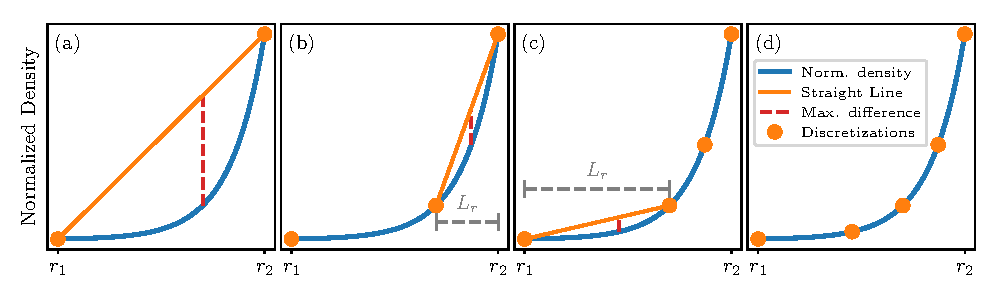
\includegraphics[width=\linewidth]{figs/tesseroids-variable-density/density-based-discretization-algorithm.pdf}
\caption{
    Ejemplo de la aplicación del algoritmo de discretización basado en densidad
    a una función densidad no lineal.
    (a)~La función densidad normalizada $\rho_n(r')$ (azul), los límites
    actuales del tesseroide (puntos naranja), y la \emph{línea recta}
    $\rho_l(r')$ (línea naranja).
    Las líneas de a trazos rojas representan la máxima diferencia de densidad
    $\Delta \rho (r')$ a la cual el tesseroide será subdividido (asumiendo que
    la desigualdad~\ref{eq:delta-density} no se satisface).
    (b)~Segunda iteración del algoritmo con una nueva \emph{línea recta}
    y máxima diferencia de densidad. El tesseroide será dividido a la
    profundidad indicada por la linea roja de a trazos.
    (c)~Tercera iteración del algoritmo.
    (d)~ Salida final del algoritmo de discretización basado en densidad,
    asumiendo que los cuatro tesseroides nuevos satisfacen la
    desigualdad~\ref{eq:delta-density}.
}
\label{fig:density-discretization-algorithm}
\end{figure}


El algoritmo puede comprenderse a través de los siguientes pasos
(Fig.~\ref{fig:density-discretization-algorithm}):

\textit{Paso 1}:
Definimos una \emph{línea recta} $\rho_l(r')$ que toma los mismos valores que
la función densidad normalizada $\rho_n(r')$ en los extremos del tesseroide
($r_1$ y $r_2$):

\begin{equation}
    \rho_l(r') =
    \frac{ \rho_n(r_2) - \rho_n(r_1) }{ r_2 - r_1 } (r' - r_1) + \rho_n(r_1).
    \label{eq:density-reference-line}
\end{equation}

\textit{Paso 2}:
Evaluamos la función de densidad normalizada y la \emph{línea recta} en un
rango de $N$ radios entre $r_1$ y $r_2$. Hemos optado por un $N = 101$, pero el
valor específico de $N$ no es crítico para el funcionamiento del algoritmo.

\textit{Paso 3}:
Calculamos la diferencia absoluta entre los valores de la \emph{línea recta}
y la función densidad normalizada:

\begin{equation}
    \Delta \rho (r') = | \rho_n(r') - \rho_l(r') |.
    \label{eq:density-abs-diff}
\end{equation}

\textit{Paso 4}:
Si la siguiente desigualdad se satisface, el tesseroide no será subdividido:

\begin{equation}
    \text{max}\{ \Delta \rho(r') \} \frac{L_r}{L_r^\text{orig}} \le \delta,
    \label{eq:delta-density}
\end{equation}

\noindent
donde $L_r$ es la dimensión radial del tesseroide considerado para ser
subdividido,

\begin{equation}
    L_r = r_2 - r_1,
\end{equation}

\noindent $L_r^\text{orig}$ es la dimensión radial del tesseroide
\emph{original}, y $\delta$ es una constante positiva que denominaremos
\emph{ratio delta}.

\textit{Paso 5}:
Si la desigualdad~\ref{eq:delta-density} no se satisface, entonces dividimos el
tesseroide en dos a una profundidad dada por el radio $r_\text{max}$ a la cual
la máxima diferencia absoluta (ec.~\ref{eq:density-abs-diff}) tiene lugar.
Repetimos los pasos 1~a~5 para cada tesseroide pequeño producido por este paso.

\textit{Paso final}:
Una vez que todos los pequeños tesseroides satisfacen la
desigualdad~\ref{eq:delta-density}, cada uno es sometido al algoritmo de
discretización adaptativa bidimensional descripto anteriormente con el objeto
de calcular sus efectos gravitatorios.

En la primer iteración, la relación $L_r/L_r^\text{orig}$ es igual a 1, ya que
el tesseroide que se considera para subdividir corresponde al \emph{original}.
En las subsiguientes iteraciones, esta relación sera progresivamente menor que
1 a medida que los tesseroides son cada vez más pequeños.
La intención de este comportamiento es limitar la cantidad de divisiones a un
numero que reduzca significativamente el error numérico:
dividir un tesseroide grande con un $\text{max}\{ \Delta \rho(r') \}$ bajo
mejoraría la precisión de la integración en mayor medida que dividiendo un
tesseroide pequeño con un $\text{max}\{ \Delta \rho(r') \}$ mayor.

A mayor valor de $\delta$, se llevarán a cabo menor cantidad de divisiones,
y viceversa.
Por ende, el valor de $\delta$ controla cuántas veces los tesseroides serán
divididos basados en la función densidad, e indirectamente, determina la
precisión y el tiempo de cómputo de la integración numérica.
Esto hace surgir la necesidad de determinar un valor máximo de $\delta$ que
garantice una precisión aceptable mientras minimiza el tiempo de cómputo.


\subsection{Resumen del algoritmo}

En resumen, dado un tesseroide con densidad variable en profundidad según una
función continua arbitraria, proponemos seguir los siguientes pasos para
calcular numéricamente sus campos gravitatorios en cualquier punto exterior:

\textit{Paso 1:}
Aplicar el \emph{algoritmo de discretización basado en densidad} para
subdividir al tesseroide a lo largo de la dirección radial, produciendo un
conjunto de tesseroides con las mismas dimensiones longitudinales
y latitudinales que el original, pero con diferentes límites radiales.

\textit{Paso 2:}
Aplicar el \emph{algoritmo de discretización adaptativa bidimensional} a cada
tesseroide obtenido en el paso anterior.
Si es necesario, el algoritmo subdividirá cada tesseroide en las direcciones
longitudinal y latitudinal, generando un conjunto de tesseroides más pequeños.

\textit{Paso 3:}
Aplicar una \ac{GLQ} de segundo orden para calcular numéricamente los campos
gravitatorios (ec.~\ref{eq:glq-var-dens}) generados por cada tesseroide
obtenido en el paso anterior. La integración numérica incluye la función
densidad y puede ser aplicada sin modificaciones a cualquier función continua.
La suma de todos estos resultas corresponde al campo gravitatorio generado por
el tesseroide original.


\subsection{Implementación por Software}

Hemos implementado los algoritmos descriptos en las secciones anteriores
mediante el uso del lenguaje de programación Python.
El software está basado en la implementación en Python de \citet{uieda2016}
incluida en la librería Fatiando a Terra v0.5 \citep{uieda2013}.
Los pasos que involucran un mayor tiempo de cómputo han sido escritos en
lenguaje Cython para alcanzar un mejor desempeño.
Aprovechamos la naturaleza dinámica del lenguaje Python para permitir funciones
de densidades definidas por el usuario o la usuaria como entradas del software.
Por ende, nuestro código puede evaluar sin modificaciones funciones lineales,
exponenciales, polinomiales, sinusoidales, splines cúbicas o cualquier otra
función de densidad continua.
Esta implementación se encuentra disponible libremente bajo la licencia
open-source BSD 3-clause.
Todo el código fuente, los scripts de Python, los datos y resultados se
encuentran disponibles a través del siguiente repositorio
\href{
    https://doi.org/10.6084/m9.figshare.8239622
}{
    doi.org/10.6084/m9.figshare.8239622
}
\citep{soler2019b} o
\href{
    https://github.com/pinga-lab/tesseroid-variable-density
}{
    github.com/pinga-lab/tesseroid-variable-density
}.
El repositorio también contiene instrucciones para replicar los resultados
presentados en este capítulo.


%%%%%%%%%%%%%%%%%%%%%%%%%%%%%%%%%%%%%%%%%%%%%%%%%%%%%%%%%%%%%%%%%%%%%%%%%%%%%

\section{Determinación de los ratio distancia-tamaño y delta}

El ratio distancia-tamaño $D$ de la discretización adaptativa y el ratio delta
$\delta$ de la discretización basada en la densidad determinan cuantas veces
cada tesseroide será dividido y por ende controlan indirectamente el error
numérico de las integraciones.
Debemos determinar valores óptimos para $D$ y $\delta$ si deseamos asegurar
tanto una precisión numérica aceptable así como una eficiencia computacional de
los algoritmos.

\citet{uieda2016} compararon los resultados de las integraciones numéricas de
tesseroides homogéneos con las soluciones analíticas de un cascarón esférico
\citep{mikuska2006, grombein2013} con el objetivo de obtener valores
predeterminados para el ratio distancia-tamaño $D$.
Seguiremos esta idea, pero en nuestro caso el cascarón esférico debe tener el
mismo perfil de densidad que nuestro modelo de tesseroides. \citet{lin2019}
obtuvieron la solución analítica del potencial gravitatorio generado por un
cascarón esférico con densidad lineal en la coordenada radial.
Aplicando el Teorema del Cascarón de Newton \citep{chandrasekhar1995,
binney2008}, podemos derivar expresiones para el potencial gravitatorio de un
cascarón esférico con densidades lineales, exponenciales o sinusoidales (ver
Apéndice~\ref{sec:shell}).

Con el objetivo de comparar los resultados numéricos con las soluciones
analíticas debemos construir modelos de un cascarón esférico a partir de
tesseroides.
Dividimos entonces el cascaron esférico a lo largo de las direcciones
longitudinales y latitudinales obteniendo un modelo de cascarón conformado por
$6 \times 12 = 72$ tesseroides de un tamaño de $30^\circ \times 30^\circ$.
Hemos definido varios modelos de cascarones con diferentes espesores
(Tabla~\ref{tab:shell-models}) para poder evaluar la discretización basada en
densidad en diferentes escenarios.
Los valores de espesor fueron elegidos para cubrir un amplio rango de
posibles aplicaciones: desde modelos topográficos a escalas litosféricas.
Dado que la cantidad de subdivisiones en la discretización adaptativa será
proporcional al tamaño de los tesseroides (ec.~\ref{eq:condition}),
algunas de estas configuraciones representan los peores casos.
La mayoría de las aplicaciones prácticas usarían tesseroides más pequeños que
$30^\circ \times 30^\circ \times 1000\ \text{km}$.

Las diferencias entre la solución analítica y los resultados numéricos pueden
ser calculados en un único punto de cómputo debido a la simetría rotacional del
cascarón esférico.
Sin embargo, los resultados numéricos dependen de la posición relativa entre el
punto de cómputo y el tesseroide \citep{ku1977, asgharzadeh2007, uieda2016}.
Tendremos en cuenta este fenómeno calculando dichas diferencias sobre grillas
regulares y almacenando únicamente la diferencia máxima absoluta.
Estos cálculos serán realizados sobre cuatro grillas diferentes
(Tabla~\ref{tab:grids}):
una grilla local sobre el polo, una grilla local en el ecuador, una grilla
global a altitud cero, y una grilla global a una altitud de 260km sobre la
superficie del cascarón (representando la altitud nominal del satélite GOCE).
Estas grillas cubren un amplio espectro de escenarios y asegurarán una
precisión aceptable para cada uno de ellos.

Las comparaciones entre las soluciones analíticas y los resultados numéricos
serán llevadas a cabo utilizando funciones de densidades lineales,
exponenciales y sinusoidales.
La densidad sinusoidal es incluida con el objetivo de evaluar la aproximación
numérica en sus límites de desempeño.
Repetimos estas comparaciones para cada combinación de modelos de tesseroides
en la Tabla~\ref{tab:shell-models} y grillas de la Tabla~\ref{tab:grids}.
A partir de estos resultados generalizaremos valores óptimos para $D$
y $\delta$ que garantizan errores numéricos menores a 0.1\% en comparación con
las soluciones analíticas del cascarón esférico en la mayoría de los casos.

\begin{table}
\caption{
    Descripción de los modelos de tesseroides utilizados para construir
    cascarones esféricos y caracterizar la precisión de las integraciones
    numéricas.
    El radio exterior ($R_2$) de cada modelo es igual al radio medio de la
    Tierra (6378.137 km), mientras que le radio interior ($R_1$) es determinado
    por el espesor del cascarón.
    La cantidad total y las dimensiones horizontales de los tesseroides en cada
    modelo de cascarón están detalladas según dimensiones latitudinales
    y longitudinales, respectivamente.
    \newline
}
\label{tab:shell-models}
\centering
\begin{tabular}{rccccc}
    Espesor & Tamaño de cada tesseroide  & Cantidad de tesseroides \\ \hline
    0.1 km  & $30^\circ \times 30^\circ$ & $6 \times 12 = 72$ \\
    1 km    & $30^\circ \times 30^\circ$ & $6 \times 12 = 72$ \\
    10 km   & $30^\circ \times 30^\circ$ & $6 \times 12 = 72$ \\
    100 km  & $30^\circ \times 30^\circ$ & $6 \times 12 = 72$ \\
    1000 km & $30^\circ \times 30^\circ$ & $6 \times 12 = 72$ \\
\end{tabular}
\end{table}

\begin{table}
\caption{
    Descripción de las grillas de putos de cómputo utilizadas para caracterizar
    la precisión de las integraciones numéricas.
    La altitud de las grillas es definida por encima del radio medio de la
    Tierra.
    \newline
}
\label{tab:grids}
\centering
\begin{tabular}{lccc}
    Nombre & Espaciado de la grilla & Región (grados) & Altitud (km)
    \\ \hline
    Polo      & $0.1^\circ$ &   0E /   1E / 89N / 90N & 0   \\
    Ecuador   & $0.1^\circ$ &   0E /   1E /  0N / 1N  & 0   \\
    Global    & $ 10^\circ$ & 180W / 180E / 90S / 90N & 0   \\
    Satélite  & $ 10^\circ$ & 180W / 180E / 90S / 90N & 260 \\
\end{tabular}
\end{table}


\subsection{Densidad Lineal}

El potencial gravitatorio y su derivada vertical que genera un cascarón
esférico con una función de densidad lineal dada por

\begin{equation}
    \rho(r') = ar' + b,
    \label{eq:density-linear}
\end{equation}

\noindent posee soluciones analíticas dadas por las
ecuaciones~\ref{eq:shell-pot-linear} y~\ref{eq:shell-gz}. Los valores de los
coeficientes $a$ y $b$ pueden ser elegidos de forma tal que la densidad asuma
valores valores iguales a  $\rho_\text{in} = 3300$\kgpercubicm{} y
$\rho_\text{out} = 2670$\kgpercubicm{} en los radios interior ($R_\text{in}$)
y exterior ($R_\text{out}$) del cascarón, respectivamente:

\begin{equation}
    a = \frac{\rho_\text{out} - \rho_\text{in}}{R_\text{out} - R_\text{in}},
\end{equation}

\begin{equation}
    b = \rho_\text{out} -
    \frac{
        \rho_\text{out} - \rho_\text{in}
    }{
        R_\text{out} - R_\text{in}
    } R_\text{out}.
\end{equation}


\begin{figure}
\centering
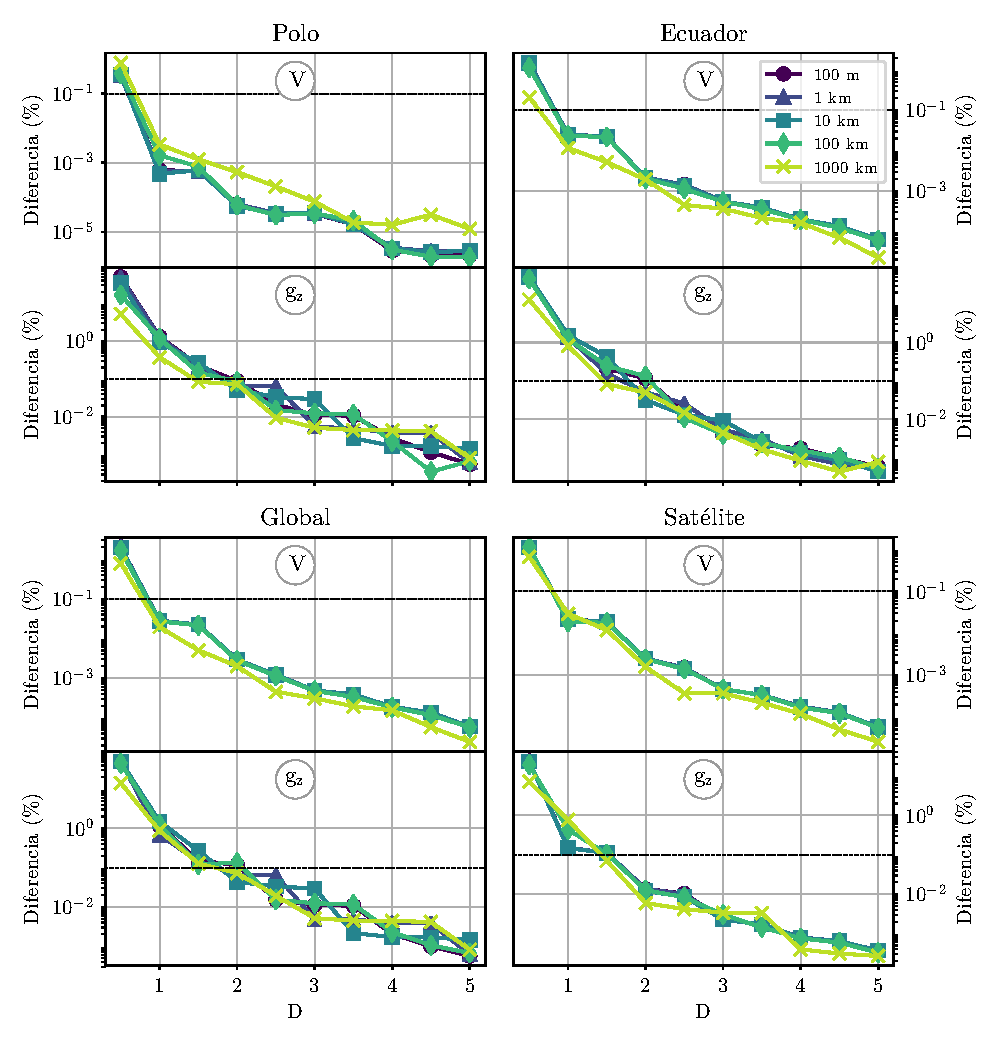
\includegraphics[width=\linewidth]{figs/tesseroids-variable-density/linear-density-diffs.pdf}
\caption{
    Diferencias entre los campos gravitatorios generados por cada modelo de
    cascarón hecho con tesseroides y sus respectivas soluciones analíticas en
    función del ratio distancia-tamaño $D$.
    Cada modelo posee una densidad lineal (ec.~\ref{eq:density-linear}).
    Los cálculos fueron realizados sobre las cuatro grillas descriptas en la
    Tabla~\ref{tab:grids}.
    Cada curva representa la diferencia máxima absoluta entre los resultados
    numéricos y las solución analítica para un dado modelo de cascarón.
    Debido a la linealidad de la función densidad, el algoritmo de
    discretización basado en densidad no es aplicado.
    Las diferencias están reportadas como un porcentaje de las soluciones
    analíticas.
    Las líneas horizontales de a trazos y color negro representan el umbral de
    precisión de 0.1\%.
}
\label{fig:D-linear}
\end{figure}

Las diferencias absolutas definidas en la ecuación~\ref{eq:density-abs-diff}
son siempre cero para cualquier tipo de densidad lineal.
Como resultado, la desigualdad~\ref{eq:delta-density} será siempre satisfecha
y no será necesario subdividir el tesseroide en la dirección radial durante la
discretización basada en densidad.
Por lo tanto, solo la discretización adaptativa bidimensional es el único
mecanismo que controla la precisión de la integración numérica para el caso de
densidad lineal.
Por esta razón ignoraremos los valores de $\delta$ y solo determinaremos el
mínimo valor de $D$ necesario para garantizar una precisión aceptable.

Calculamos el potencial gravitatorio ($V$) y su derivada vertical ($g_z$)
para cada modelo de cascarón esférico definido en la
Tabla~\ref{tab:shell-models} en cada grilla de cómputo de la
Tabla~\ref{tab:grids}.
Las derivadas horizontales del potencial son iguales a cero fuera del cascarón
debido a la simetría rotacional, y por ende son omitidos del análisis.
Estos cálculos son repetidos para valores de ratio distancia-tamaño $D$ desde
0.5 a 5 con incrementos de 0.5.
Luego calculamos la diferencia absoluta entre los resultados numéricos y las
soluciones analíticas para el cascarón.
La Figura~\ref{fig:D-linear} muestra la máxima diferencia absoluta para cada
modelo de cascarón y grilla de cómputo como función de $D$.
Las diferencias se muestran relativas a la solución analítica para cada
cascarón.
Finalmente, seleccionamos el valor óptimo de $D$ como el menor valor para el
cual la diferencia es menor a 0.1\%.

A partir de la Figura~\ref{fig:D-linear} podemos observar que los errores
relativos para el potencial $V$ y para su derivada vertical $g_z$ caen por
debajo del umbral de 0.1\% para valores de $D=1$ y $D=2.5$, respectivamente.
Notablemente, un valor de $D=2$ sería suficiente para $g_z$ en el caso de una
grilla a altitud satelital.
Para el resto de las configuraciones, dichos valores son consistentes
e independientes del espesor de cascarón o de la ubicación geográfica.


\subsection{Densidad exponencial}

Para una función de densidad exponencial, la discretización basada en densidad
será aplicada con anterioridad al algoritmo de discretización adaptativa.
Esto significa que los valores óptimos para el ratio distancia-tamaño $D$ y el
ratio delta $\delta$ (ec.~\ref{eq:delta-density}) deben ser determinados
simultáneamente.
Para ello llevamos a cabo un análisis de error similar al que aplicamos en el
caso de densidad lineal.
Ahora el cascarón esférico poseerá una densidad según una función exponencial
que asume los valores de $\rho_\text{out} = 2670$\kgpercubicm{}
y $\rho_\text{in} = 3300$\kgpercubicm{} en las superficies externas
e internas, respectivamente, y que se define de la siguiente manera:

\begin{equation}
    \rho(r') = A e^{- b \frac{r' - R_1}{R_2 - R_1}} + C,
    \label{eq:density-exp}
\end{equation}

\noindent donde

\begin{equation}
    A = \frac{\rho_\text{in} - \rho_\text{out}}{1 - e^{-b}},
\end{equation}

\begin{equation}
    C = \rho_\text{in} - A,
\end{equation}

\noindent y $b$ es una constante adimensional que determina el grado de
variabilidad de la función. Un valor mayor de $b$ aumenta la máxima pendiente
de la función densidad (Fig.~\ref{fig:exp-densities}).

\begin{figure}
\centering
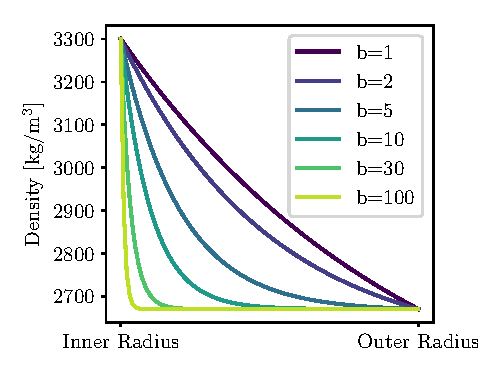
\includegraphics[width=0.5\linewidth]{figs/tesseroids-variable-density/exponential-densities.pdf}
\caption{
    Funciones de densidad exponencial asignadas a los modelos de cascarón
    esférico para la determinación del ratio $\delta$.
    Cada función densidad corresponde a diferentes valores de $b$ en la
    ecuación~\ref{eq:density-exp}.
}
\label{fig:exp-densities}
\end{figure}


\subsubsection{Exploración del espacio $D$-$\delta$}

Nuestro objetivo es hallar una combinación de valores para $D$ y $\delta$ que
produzcan un error numérico menor al umbral de 0.1\% mientras minimicen el
tiempo de cómputo.
Para ello hacemos uso del método de búsqueda en grilla (\emph{grid search} en
inglés) y calculamos el error numérico para cada par ($D$, $\delta$)
perteneciente a una grilla en el espacio $D$-$\delta$
(Fig.~\ref{fig:grid-search}).
Con el objeto de obtener un óptimo desempeño del algoritmo, buscamos el ($D$,
$\delta$) que minimice el número de subdivisiones de tesseroides mientras
mantengan el error numérico por debajo del umbral de 0.1\%.
Este requisito se traduce en minimizar el valor de $D$ y maximizar el valor de
$\delta$.

Dado que la búsqueda en grilla es un proceso computacionalmente costoso,
limitamos el análisis a un valor alto de $b=30$ (Fig.\ref{fig:exp-densities})
y la grilla de cómputo \emph{Global} definida en la Tabla~\ref{tab:grids}.
Calculamos la diferencia relativa entre el resultado numérico y la solución
analítica del potencial gravitatorio ($V$) y su derivada vertical ($g_z$) para
cada modelo de cascarón definido en la Tabla~\ref{tab:shell-models}.
La Figura~\ref{fig:grid-search} muestra la máxima diferencia obtenida para
todos los modelos de cascarón.
Las líneas de a trazos representan un contorno correspondiente al 0.1\% de
error relativo, por ende los puntos interiores a ella son los que caen debajo
de dicho umbral.
Además, la figura destaca los valores de $D$ obtenidos en la sección anterior
para el caso de densidad lineal ($D_\text{linear}$).

Los valores más chicos de $D$ que se encuentran debajo del umbral de 0.1\%
coinciden con los valores $D_\text{linear}$ tanto para $V$ como para $g_z$.
Estos resultados indican que los valores de $D_\text{linear}$ obtenidos pueden
ser extrapolados a los casos de densidades no lineales.
Esto no es una sorpresa, ya que la discretización adaptativa bidimensional y la
discretización basada en densidad son independientes una de la otra.
La primera divide al tesseroide en las direcciones horizontales, mientras que
la otra lo hace solo en la dirección radial.
Por ende, es de esperar que el valor óptimo de $\delta$ sea independiente del
valor óptimo de $D$.
Dado que la búsqueda en grilla fue limitada a una grilla de cómputo específica
y a un único valor de $b$, en la próxima sección realizaremos un análisis más
detallado para determinar un valor óptimo de $\delta$ para el caso de densidad
exponencial.

\begin{figure}
\centering
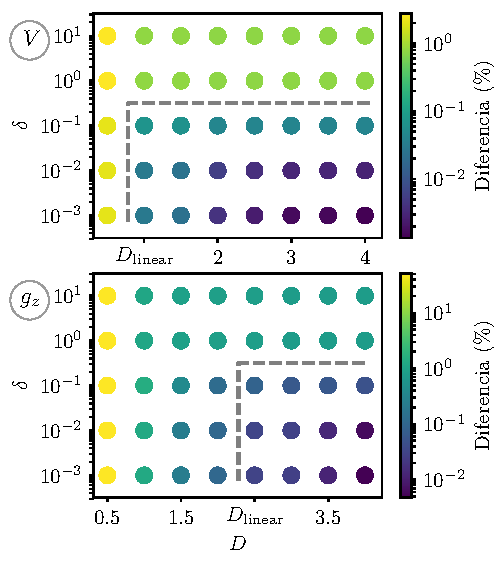
\includegraphics[width=0.5\linewidth]{figs/tesseroids-variable-density/grid-search.pdf}
\caption{
    Exploración del error numérico en el espacio $D$-$\delta$.
    Los valores porcentuales de diferencia fueron obtenidos a partir de la
    comparación entre las soluciones analíticas y las aproximaciones numéricas
    de los campos gravitatorios ($V$ y $g_z$) generados por un cascarón
    esférico con una densidad exponencial
    (ec.~\ref{eq:density-exp}) con $b=30$.
    Estas comparaciones fueron realizadas sobre la grilla de cómputo
    \emph{Global} (Tabla~\ref{tab:grids}), con los modelos de cascarón
    esféricos detallados en la Tabla~\ref{tab:shell-models}.
    Los valores de diferencias porcentuales fueron obtenidos como la máxima
    diferencia de entre todos los modelos de cascarón.
    Los puntos interiores a la región delimitada por las lineas de a trazos son
    los que presentan un error por debajo del umbral de 0.1\%.
    Los valores de $D$ obtenidos para el caso de densidad lineal para cada
    campo gravitatorio se encuentran identificados con $D_\text{linear}$.
    }
\label{fig:grid-search}
\end{figure}


\subsubsection{Determinación del ratio delta}

Habiendo fijado valores de $D$ iguales a los obtenidos para el caso de
densidad lineal, nos encontramos en condiciones de explorar los errores de
integración como función de $\delta$ en mayor detalle.
Calcularemos la diferencia entre el error numérico y las soluciones analítica
para todas las combinaciones de grillas de cómputo (Tabla~\ref{tab:grids})
y modelos de cascarón esférico (Tabla~\ref{tab:shell-models}),
variando los valores de $\delta$ entre $10^{-3}$ y $10^{1}$.
Los cálculos son repetidos para cada valor de $b \in \{1, 2, 5, 10, 30, 100\}$
(Fig.~\ref{fig:exp-densities}) con el objeto de analizar la precisión del
método para diversos tipos de funciones exponenciales.
Dado que valores mayores de $\delta$ producen menores subdivisiones, nuestra
intención es hallar los valores máximos de $\delta$ que producen una diferencia
relativa por debajo del umbral de 0.1\%.
La Figura~\ref{fig:delta-exponential} muestra las diferencias relativas
resultantes para $V$ y $g_z$ como función de $\delta$.
Por brevedad, cada curva corresponde a la diferencia máxima entre todos los
modelos de cascarón esférico.
Las curvas correspondientes a $b=1$ y $b=2$ se encuentran por debajo del umbral
0.1\% para todos los valores de $\delta$ y no se ven modificadas para valores
de $\delta > 0.8$, indicando que esas funciones de densidad son los
suficientemente suaves como para poder prescindir de discretizaciones en la
dirección radial.
Para todos los otros valores de $b$, las diferencias caen debajo del umbral si
$\delta=0.1$.
Estos resultados indican que no hay una relación significativa entre la
suavidad de la densidad exponencial y el error numérico.

\begin{figure}
\centering
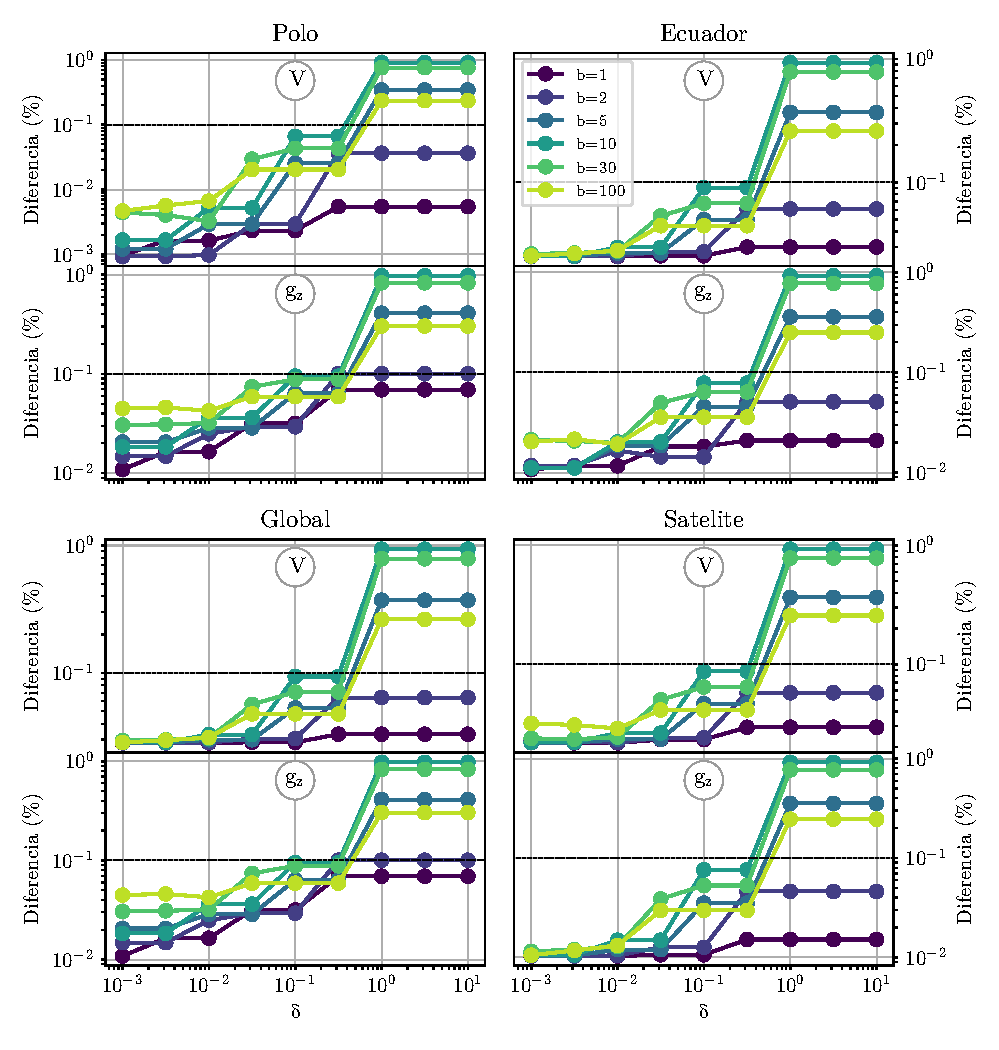
\includegraphics[width=\linewidth]{figs/tesseroids-variable-density/exponential-density-diffs.pdf}
\caption{
    Diferencias entre el error numérico y las soluciones analíticas como
    función del ratio $\delta$ para varias funciones de densidad exponenciales.
    Estas comparaciones fueron llevadas a cabo para cada combinación entre los
    modelos de cascarón (Tabla~\ref{tab:shell-models}) y las grillas de cómputo
    (Tabla~\ref{tab:grids}) haciendo uso de un valor fijo de $D$. Cada curva
    corresponde a la diferencia máxima obtenida para cada modelo de cascarón
    para un valor particular de $b$ (ec.~\ref{eq:density-exp}). Las diferencias
    están reportadas como un porcentaje de las soluciones analíticas. Las
    líneas horizontales de a trazos y color negro representan el umbral de
    precisión de 0.1\%.
    }
\label{fig:delta-exponential}
\end{figure}


\subsection{Densidad sinusoidal}

Hasta ahora hemos analizado el comportamiento de la discretización basada en
densidad contra funciones de densidades lineales y exponenciales.
Sin embargo, este nuevo algoritmo es adecuado para ser utilizado con funciones
continuas más complejas, por ejemplo funciones no monotónicas o que presenten
múltiples puntos de inflexión.
Aunque este tipo de funciones de densidad son cuanto mucho raras de encontrar
en seteos geológicos, queremos someter nuestro algoritmo a estos casos con el
objetivo de mostrar de que puede resolver situaciones más complejas que
funciones lineales y exponenciales.
Además, obtener un valor óptimo del ratio $\delta$ para casos de funciones de
densidades irreales nos permitiría extrapolarlo a casos más simples
y realistas.
Es por esta razón que los análisis que se describirán a continuación están
destinados a someter el algoritmo a sus extremos y no para emular un escenario
real.

Consideremos modelos de cascarones específicos con una función de densidad
sinusoidal que se define de la siguiente manera:

\begin{equation}
    \rho(r') = A \sin \left( 2 \pi b \frac{r' - R}{R_2 - R_1} \right) + A,
    \label{eq:density-sine}
\end{equation}

\noindent donde $A$ es una constante que controla la amplitud y la traslación
vertical de la función seno, $R$ es el radio medio de la Tierra y $b$ es una
constante adimensional que regula cuántos períodos de la función trigonométrica
serán incluidos dentro de los radios interior y exterior.
La solución analítica para el potencial $V$ y su gradiente vertical $g_z$ que
genera un cascarón esférico con una densidad sinusoidal puede hallarse en el
Apéndice~\ref{sec:shell}.

Calculamos la diferencia relativa entre los resultados numéricos y la solución
analítica para $V$ y $g_z$ para cada combinación de modelos de cascarones
(Tabla~\ref{tab:shell-models}) y grillas de cómputo (Tabla~\ref{tab:grids}).
Hemos fijado el ratio distancia-tamaño $D$ a los valores obtenidos para el caso
de densidad lineal y exploramos valores de $\delta$ entre $10^{-4}$ y $1$. Los
cálculos fueron repetidos para valores de $b$ iguales a 1, 2, 5 y 10.
(Fig.~\ref{fig:sine-densities}). En todos los casos el valor de $A$ fue fijado
a 1650\kgpercubicm{}.

\begin{figure}
\centering
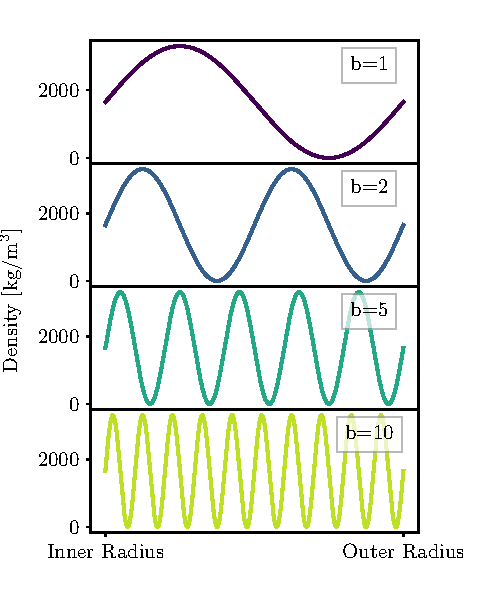
\includegraphics[width=0.5\linewidth]{figs/tesseroids-variable-density/sine-densities.pdf}
\caption{
    Densidades sinusoidales asignadas a los cascarones esféricos durante la
    determinación del ratio $\delta$. Cada función de densidad corresponde a un
    valor distinto de $b$ en la ecuación~\ref{eq:density-sine}.
}
\label{fig:sine-densities}
\end{figure}

\begin{figure}
\centering
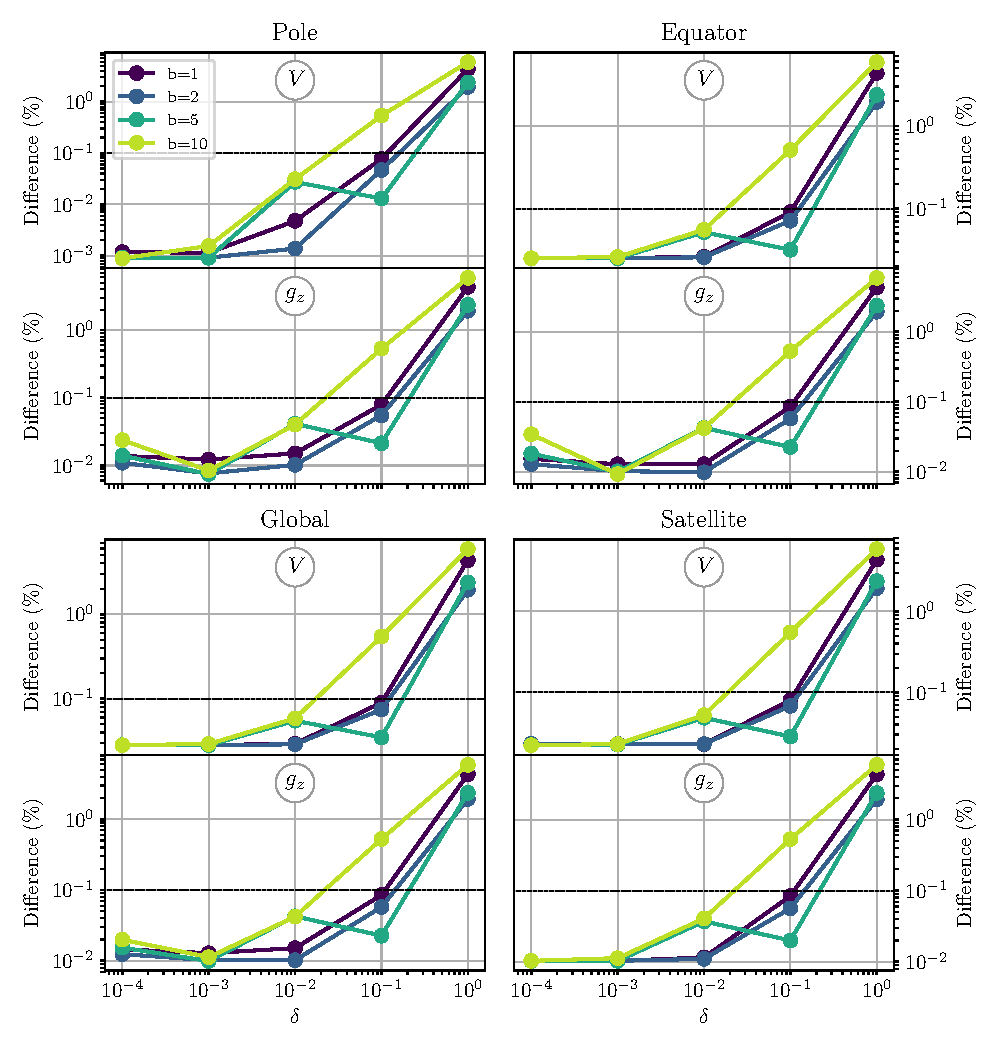
\includegraphics[width=\linewidth]{figs/tesseroids-variable-density/sine-density-diffs.pdf}
\caption{
    Diferencias entre los resultados numéricos y las soluciones analíticas como
    función de $\delta$ para diferentes funciones de densidad sinusoidales.
    Las comparaciones fueron llevadas a cabo para cada modelo de cascarón
    (Tabla~\ref{tab:shell-models}) y cada grilla de cómputo
    (Tabla~\ref{tab:grids}) haciendo uso de un valor fijo de $D$.
    Cada curva corresponde a la diferencia máxima obtenida para cada modelo de
    cascarón para un valor particular de $b$ (ec.~\ref{eq:density-sine}).
    Las diferencias están reportadas como un porcentaje de las soluciones
    analíticas. Las líneas horizontales de a trazos y color negro representan
    el umbral de precisión de 0.1\%.
    }
\label{fig:delta-sine}
\end{figure}

La Figura~\ref{fig:delta-sine}
muestra las diferencias relativas entre los resultados numéricos y las
soluciones analíticas para casos de densidades sinusoidales.
Nuevamente, cada curva corresponde a la diferencia máxima para cada modelo de
cascarón.
Para todos los valores de $b$, a excepción de $b=10$, las diferencias caen
debajo del umbral 0.1\% para $\delta = 0.1$.
En el caso de $b=10$, un menor valor de $\delta = 0.01$ es necesario para
alcanzar dicho umbral.
Vale notar que incluso para el caso de $b=10$, las diferencias obtenidas
utilizando $\delta = 0.1$ se encuentran debajo del 1\%.


%%%%%%%%%%%%%%%%%%%%%%%%%%%%%%%%%%%%%%%%%%%%%%%%%%%%%%%%%%%%%%%%%%%%%%%%%%%%%%%

\section{Desempeño del algoritmo}

Dado que el algoritmo de discretización basada en densidad introduce
subdivisiones a lo largo de la dirección radial, es razonable suponer que el
tiempo de cómputo para el caso de densidades variables será más alto que en el
caso de densidades homogéneas.
Comparar directamente el tiempo de cómputo en ambos casos no podría ser
realizado de forma significativa, ya que dependería fuertemente en la
implementación del algoritmo, la elección del lenguaje de programación y la
función densidad en particular.
Con el objetivo de obtener un indicador sobre cuánto aumenta el costo
computacional, elegimos la cantidad de subdivisiones al tesseroides en la
discretización basada en densidad como una variable proxy.

Analizamos densidades exponenciales (ec.~\ref{eq:density-exp}) con valores de
$b$ iguales a 1, 2, 5, 10, 30 y 100, y densidades sinusoidales
(ec.~\ref{eq:density-sine}) con valores de $b$ iguales a 1, 2, 5, y 10.
Aplicamos el algoritmo de discretización basado en densidad sobre cada una de
esas funciones y registramos la cantidad de divisiones que produce en cada
caso.
Las Figuras.~\ref{fig:number-of-tesseroids}a y~\ref{fig:number-of-tesseroids}b
muestran las densidades exponenciales y sinusoidales junto con sus
correspondientes puntos de discretización como círculos naranja.

En el caso de densidad exponencial, el algoritmo realiza una única subdivisión
independientemente del valor de $b$.
Por lo tanto, el tiempo de cómputo podría estimarse como el doble del caso de
una densidad homogénea (asumiendo implementaciones idénticas).
Por otro lado, la Figura~\ref{fig:number-of-tesseroids}c muestra una relación
casi lineal entre el número de divisiones para el caso de densidad sinusoidal
y los valores de $b$.
Por lo tanto, el tiempo de cómputo en estos casos parece depender de la
cantidad de períodos de la función sinusoidal contenidos dentro de los límites
del tesseroide.

\begin{figure}
\centering
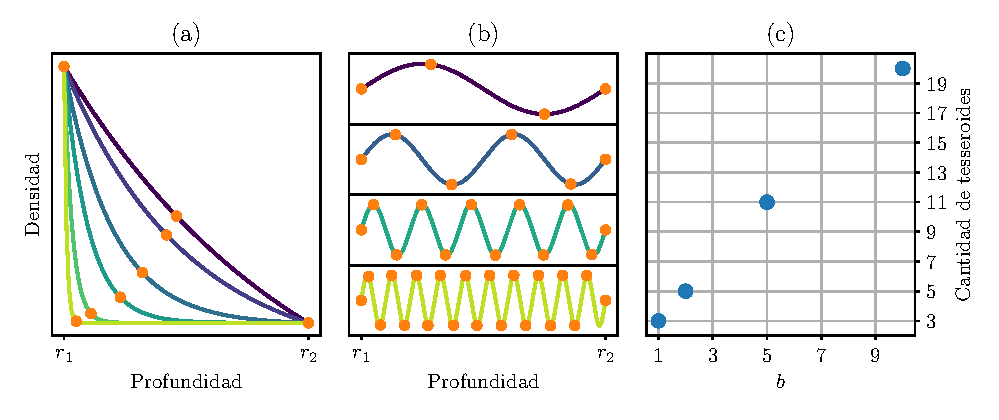
\includegraphics[width=\linewidth]{figs/tesseroids-variable-density/number-of-tesseroids.pdf}
\caption{
    Cantidad de subdivisiones realizadas por el algoritmo de discretización
    basada en densidad (con $\delta = 0.1$) en caso de
    (a)~funciones de densidad exponencial con los mismos valores de $b$
    presentes en la Fig.~\ref{fig:exp-densities},
    (b)~funciones de densidad sinusoidal con los mismos valores de $b$
    presentes en la Fig.~\ref{fig:sine-densities}.
    En ambas figuras, las ubicaciones de las discretizaciones están marcadas
    con círculos naranja.
    (c)~Muestra la cantidad de tesseroides obtenidos en el caso de densidad
    sinusoidal como función de $b$.
}
\label{fig:number-of-tesseroids}
\end{figure}


%%%%%%%%%%%%%%%%%%%%%%%%%%%%%%%%%%%%%%%%%%%%%%%%%%%%%%%%%%%%%%%%%%%%%%%%%%%%%%%

\section{Aplicación a la Cuenca Neuquina}

Hemos aplicado los nuevos algoritmos y los valores óptimos para $D$
y $\delta$ determinados previamente para calcular los efectos gravitatorios de
la Cuenca Neuquina, una cuenca sedimentaria localizada al este de los Andes,
entre las latitudes 32$^\circ$S y 40$^\circ$S (Fig.~\ref{fig:neuquen-basin}a).
La cuenca incluye siliciclástos marinos y sedimentarios, carbonatos
y evaporitas acumuladas durante el Jurásico y el Cretácito constituyendo un
registro estratigráfico hasta 5000m de profundidad \citep{howell2005}.

\begin{figure}
\centering
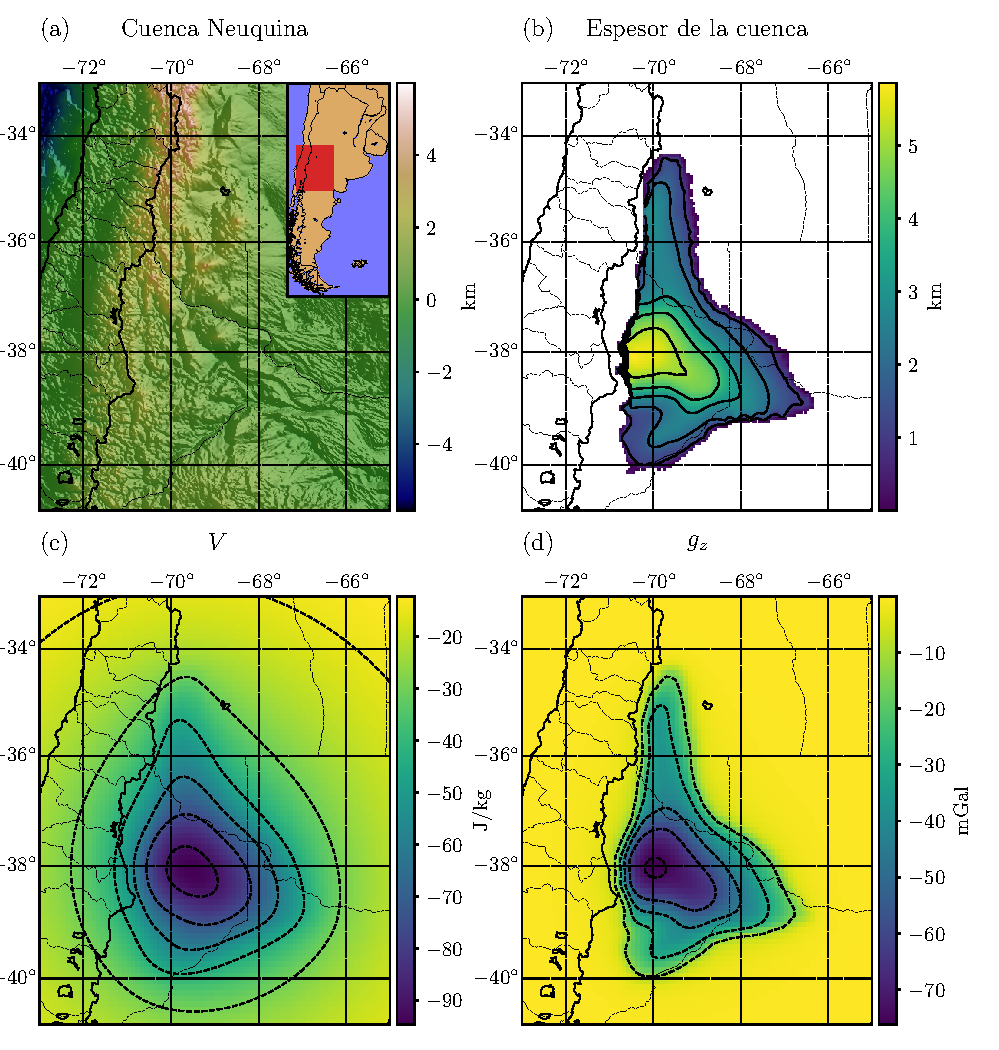
\includegraphics[width=\linewidth]{figs/tesseroids-variable-density/neuquen-basin.pdf}
\caption{
    Efectos gravitatorios de la Cuenca Neuquina modelada utilizando tesseroides
    con una densidad exponencial como función de la profundidad.
    (a)~Topografía de la Cuenca Neuquina (en km) y su ubicación geográfica en
    Sudamérica,
    (b)~espesor de la cuenca sedimentaria \citep[en metros;][]{heine2007}
    (c)~potencial gravitatorio resultante $V$,
    (d)~componente vertical del gradiente ($g_z$),
    calculadas a 10km de altitud sobre el radio medio de la Tierra.
}
\label{fig:neuquen-basin}
\end{figure}

\begin{figure}
\centering
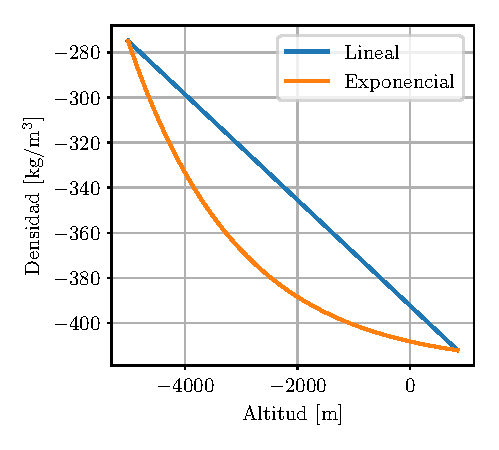
\includegraphics[width=0.5\linewidth]{figs/tesseroids-variable-density/neuquen-basin-densities.pdf}
\caption{
    Densidades lineales y exponenciales utilizadas para el cálculo de los
    campos gravitacionales generados por un modelo de la Cuenca Neuquina
    compuesto por tesseroides.
    La altitud se define por encima del radio medio de la Tierra, y sus eje se
    extiende entre el puntos más profundo hasta el punto más alto de la cuenca.
}
\label{fig:neuquen-basin-densities}
\end{figure}


\begin{figure}
\centering
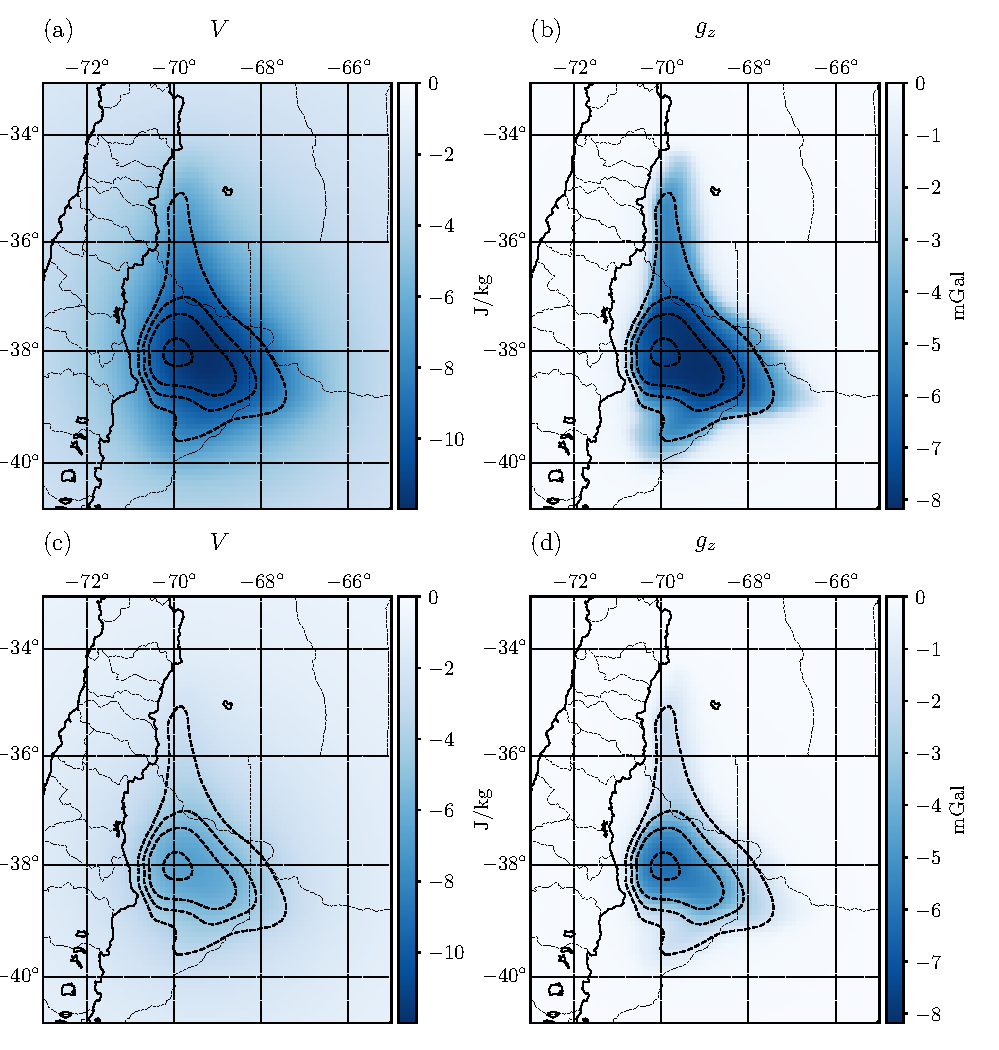
\includegraphics[width=\linewidth]{figs/tesseroids-variable-density/neuquen-basin-diffs.pdf}
\caption{
    Diferencias entre los campos gravitatorios generados por el modelo de
    tesseroides de la Cuenca Neuquina con una densidad exponencial y con el
    mismo modelo pero con densidades homogéneas y lineales.
    \mbox{(a)-(b)}~Diferencias de $V$ y $g_z$ entre el modelo con densidad
    exponencial y el modelo con densidad homogénea,
    \mbox{(c)-(f)}~diferencias de $V$ y $g_z$ entre el modelo con densidad
    exponencial y el modelo con densidad lineal,
    calculadas a 10km de altitud sobre el radio medio de la Tierra.
}
\label{fig:neuquen-basin-diffs}
\end{figure}

El espesor del paquete sedimentario fue digitalizado a partir de
\citet{heine2007} sobre una grilla regular con una resolución de 0.05$^\circ$
en las direcciones longitudinal y latitudinal (Fig.~\ref{fig:neuquen-basin}b).
Creamos un modelo del paquete sedimentario a partir de tesseroides de
$0.05^\circ \times 0.05^\circ$ ubicados sobre cada nodo de la grilla.
El límite superior de cada tesseroide fue fijado a al altitud media de la
topografía de la cuenca (845\m{} sobre el radio medio de la Tierra) y el límite
inferior es seleccionado de forma tal que cada tesseroide posea la misma
dimensión que el espesor de la cuenca sobre el correspondiente punto de la
grilla.

Además debemos definir una función densidad para el modelo de tesseroides.
\citet{sigismondi2012} determinó valores mínimos y máximos para el contraste de
densidad de la Cuenca Neuquina de -412\kgpercubicm{} y -275\kgpercubicm{},
respectivamente.
Hemos elegido una variación de densidad exponencial (ec.~\ref{eq:density-exp})
que asume el valor mínimo en la superficie superior y un valor máximo a una
profundidad de 5014\m{} (la región más profunda de la cuenca), con un valor de
$b$ igual a 3.
Esta variación de densidad se encuentran dentro de los ordenes de magnitud
utilizados por \citet{cowie1990} y \citet{cordell1973}.
La función de densidad se muestra en la
Figura~\ref{fig:neuquen-basin-densities}.

Finalmente, hemos calculado el potencial gravitatorio $V$ y la componente
vertical de su gradiente ($g_z$) sobre una grilla de cómputo compuesta por
$159\times163$ nodos (un espaciado de $0.05^\circ$ en las direcciones
longitudinal y latitudinal) a una altitud de 10\km{} sobre el radio medio de la
Tierra.
Los campos resultantes pueden apreciarse en las
Figuras~\ref{fig:neuquen-basin}c-d.

Calculamos las diferencias entre los resultados para la densidad exponencial
y para aquellos generados por el mismo modelo pero con una densidad constante
dada por el valor medio entre -412\kgpercubicm{} y -275\kgpercubicm{}.
Además calculamos las diferencias entre el modelo de densidad exponencial y uno
con densidad lineal que asume estos dos valores en los puntos más altos y más
profundos de la cuenca (Fig.~\ref{fig:neuquen-basin-densities}).
Las Figuras~\ref{fig:neuquen-basin-diffs}a-b
y ~\ref{fig:neuquen-basin-diffs}c-d muestran las diferencias con las densidad
constante y con la densidad lineal, respectivamente.
La diferencia máxima absoluta en los campos $g_z$ es aproximadamente de
8\mGal{} para el caso de densidad homogénea y aproximadamente de 6\mGal{} para
el caso lineal.
Estas discrepancias se encuentra bien por encima de los errores de la mayoría
de los relevamientos gravimétricos.


%%%%%%%%%%%%%%%%%%%%%%%%%%%%%%%%%%%%%%%%%%%%%%%%%%%%%%%%%%%%%%%%%%%%%%%%%%%%%%%

\section{Discusión}

Al incluir la función densidad dentro de la \ac{GLQ}, el método aquí descripto
puede ser aplicado sin ninguna modificación a cualquier tesseroide cuya
densidad puede representarse por una función continua en la dirección radial.
El algoritmo de discretización basado en la densidad divide el tesseroide a lo
largo de la dirección radial con el objetivo de garantizar una precisa
integración.
Este algoritmo es independiente de la integración \ac{GLQ} y puede
potencialmente ser aplicado para determinar una óptima discretización a la hora
de aproximar una función mediante funciones lineales de a pasos \citep{lin2019}
o funciones polinomiales de a paso \citep{fukushima2018}.

Nuestros resultados experimentales muestran que la discretización adaptativa
bidimensional es suficiente para alcanzar errores debajo del 0.1\% en conjunto
con una \ac{GLQ} de segundo orden en caso de densidades lineales
(Fig.~\ref{fig:D-linear}).
Los valores del ratio distancia-tamaño determinados para el
potencial gravitatorio
($D=1$)
y para su derivada vertical ($D=2.5$) son compatibles por los valores
determinados por \citet{uieda2016}.
Estos resultados muestran además que no existe una relación significativa entre
la precisión del método y el espesor del modelo de tesseroides.

La exploración del espacio $D$-$\delta$ para el caso de una densidad
exponencial (Fig.~\ref{fig:grid-search}) muestra que los valores de $D$
determinados para el caso lineal son igualmente válidos para ser aplicados al
caso exponencial.
Además, las diferencias con respecto a las soluciones analíticas caen por
debajo del umbral de 0.1\% solo para valores de $\delta$ menores a 0.1.
Por lo tanto, la aplicación de la discretización basada en la densidad es
necesaria para alcanzar el nivel de precisión deseada para el caso de
densidades no lineales.

Un análisis de errores más detallados muestra que el valor de $\delta = 0.1$ es
suficiente para garantizar errores por debajo del 0.1\% para cualquiera de las
funciones exponenciales (Fig.~\ref{fig:delta-exponential}) y para la mayoría de
las funciones sinusoidales (Fig.~\ref{fig:delta-sine}) que aquí se han probado.
La excepción se presenta en el caso de una función sinusoidal con $b = 10$
(ec.~\ref{eq:density-sine}),
para la cual un valor de $\delta = 0.01$ es necesario para alcanzar el umbral
0.1\%.
Sin embargo, utilizar un valor de $\delta = 0.1$ en este caso produce
resultados con errores por debajo del 1\%.

Aunque los algoritmos aquí propuesto pueden ser aplicados a cualquier función
de densidad continua, los valores óptimos de $D$ y $\delta$ fueron
empíricamente determinados solo para funciones lineales, exponenciales
y sinusoidales.
Por lo tanto, solo podemos afirmar con certeza que estos valores producen
resultados con errores por debajo de 0.1\% para los tipos de funciones
nombradas.
Sin embargo, todas las experiencias numéricas incluyen los escenarios menos
favorables (puntos de cómputo sobre la superficie de los tesseroides,
tesseroides de gran tamaño, funciones densidad altamente variables, etc.).
Por esta razón, es plausible extrapolar los valores óptimos de $D$ y $\delta$
a cualquier densidad continua que represente variaciones realistas de
estructuras geológicas.
A pesar de esto, alentamos a los usuarios y usuarias de estos algoritmos
a llevar a cabo experimentaciones similares con el objetivo de evaluar su
precisión en caso de utilizar funciones de densidades más complejas que las
probadas aquí.

El análisis del desempeño del algoritmo muestra que el tiempo de cómputo
en los casos de densidades variables es como mínimo el doble del
necesario para el caso de densidad homogénea o lineal.
Esta proporcionalidad puede aumentar con la cantidad de puntos de inflexión de
la función densidad.
Como en la mayoría de los métodos numéricos, existe un compromiso entre tiempo
de cómputo y precisión.
Sin embargo, los perfiles de densidad suelen tener pocos puntos de inflexión en
la mayoría de las aplicaciones geofísicas.
Por lo tanto, el tiempo de cómputo se encontrará en el mismo orden de magnitud
que el caso de densidad homogénea para la mayoría de las aplicaciones en el
mundo real.

%%%%%%%%%%%%%%%%%%%%%%%%%%%%%%%%%%%%%%%%%%%%%%%%%%%%%%%%%%%%%%%%%%%%%%%%%%%%%%%

\section{Conclusiones}

Hemos desarrollado una nueva metodología para calcular el potencial
gravitatorio y su gradiente generados por un tesseroide con una densidad dada
por una función continua de la coordenada radial.
Este método resuelve numéricamente integrales volumétricas mediante la
\ac{GLQ} incluyendo la función densidad dentro del integrando.
Mediante una implementación del algoritmo en lenguaje Python, los usuarios
y las usuarias pueden definir su propia función densidad y servirla como
entrada al algoritmo.
Esto permite el uso de funciones continuas arbitrarias sin necesidad de
realizar modificaciones sobre el método o el software.
La precisión de la integración numérica es controlada automáticamente por un
algoritmo de discretización adaptativa bidimensional y un nuevo algoritmo de
discretización basado en densidad.
El primero subdivide iterativamente al tesseroide en caso de que las relaciones
entre la distancia al punto de cómputo y las dimensiones longitudinal
y latitudinal del tesseroide sean menores que un ratio distancia-tamaño $D$
predefinido.
Este algoritmo minimiza los errores de integración a cuando el punto de
cómputo se encuentra cerca del tesseroide.
Sin embargo, la discretización adaptativa por sí sola no es suficiente para
garantizar una precisión aceptable en caso de tesseroides con densidades no
lineales.
Para solucionar esto, el algoritmo de discretización basada en densidad divide
al tesseroide a lo largo de la dirección radial en los lugares donde la
\emph{máxima variación} de la función densidad ocurre.
La cantidad de subdivisiones a lo largo del radio, y por ende la precisión del
cómputo, están controladas por el parámetro delta $\delta$.
Este nuevo algoritmo está diseñado para minimizar el error debido a la
incapacidad de la \ac{GLQ} de producir aproximaciones precisas en caso de
funciones de densidad con variaciones pronunciadas.

Hemos determinado de manera empírica valores óptimos para los parámetros $D$
y $\delta$ comparando los resultados numéricos con soluciones analíticas para
cascarones esféricos.
Nuestro análisis incluye un rango de modelos de tesseroides y grillas de
cómputo así como funciones de densidades de las más utilizadas en problemas
reales.
Estos valores minimizan el tiempo de cómputo mientras mantienen el error
numérico por debajo de un umbral de 0.1\%.
Las funciones de densidad utilizadas para establecer estos valores óptimos
fueron lineales, exponenciales y sinusoidales.
La función lineal representa la variación más sencilla de densidad y no
requiere la aplicación de una discretización basada en densidad.
Mediante este análisis hemos obtenido valores óptimos para el ratio
distancia-tamaño $D$ de 1 y 2.5 para el potencial gravitatorio y para su
gradiente, respectivamente.
Con el objetivo de analizar la precisión de la discretización basada en
densidad, hemos calculado el error numérico para casos de densidades
exponenciales, desde funciones suaves hasta funciones con fuertes pendientes,
e incluso para funciones sinusoidales de diferentes longitudes de onda.
Vale notar que la densidad sinusoidal fue tomada en cuenta con la intención de
someter al algoritmo a sus extremos y no para emular escenarios de la vida
real.
Valores de $\delta$ iguales a 0.1 son suficientes para garantizar errores
numéricos por debajo del umbral de 0.1\% para la mayoría de los casos
examinados.
Estos resultados podrían ser extrapolados a otras funciones continuas de
densidad que sean lo suficientemente suaves. Tal y como es el caso de la
mayoría de las aplicaciones geofísicas.
Menores valores de $\delta$ pueden ser utilizados para densidades altamente
variables con el objetivo de incrementar la precisión de la integración.

Una parte del desempeño y eficiencia computacional es sacrificada con el objeto
de obtener un método preciso y de propósito general.
La discretización basada en densidad aumenta el tiempo de cómputo al
incrementar el número de integraciones según la \ac{GLQ}.
De la misma manera, permitiendo a los usuarios y las usuarias elegir sus
propias funciones de densidad incurrimos en un aumento del costo computacional
debido a las subsecuentes evaluaciones de dichas funciones.
Además, resulta imposible optimizar el código fuente y la formulación
matemática para el caso general donde no conocemos las especificidades de la
función densidad.
Sin embargo, la discretización basada en densidad es independiente de la
discretización adaptativa y de la \ac{GLQ}.
Es decir, podemos tomar a este algoritmo como un preprocesado que luego puede
ser combinado con métodos de integración más específicos.

La aplicación de este algoritmo al modelado de la Cuenca Neuquina, Argentina,
demuestra que los efectos de la compactación sedimentaria no deben ser
ignorados.
Los resultados producidos por una densidad exponencial muestran un error de
8\mGal{} con respecto al caso de una densidad homogénea, y un error de 6\mGal{}
con respecto a una función lineal.
Los modelos directos robustos son una componente clave para cualquier método de
inversión de datos gravimétricos.
Y errores de esta magnitud pueden resultar en una significativa sobreestimación
del espesor del paquete sedimentario, por poner un ejemplo.


%%%%%%%%%%%%%%%%%%%%%%%%%%%%%%%%%%%%%%%%%%%%%%%%%%%%%%%%%%%%%%%%%%%%%%%%%%%%%%%

\begin{subappendices}

\section{Soluciones analíticas para un cascarón esférico}
\label{sec:shell}

Consideremos un cascarón esférico con radio interior $R_1$ y radio exterior
$R_2$, cuya densidad es función $\rho(r')$ de la coordenada radial.
Deseamos obtener una expresión analítica para los campos gravitatorios que
general en cualquier punto externo ubicado a una distancia $r$ del centro del
cascarón ($r > R_2$).

Según el Teorema del Cascarón de Newton (\emph{Newton's Shell Theorem, Theorem
XXXI}) \citep{chandrasekhar1995, binney2008}, el potencial gravitatorio
generado por el cascarón esférico en cualquier punto externo es equivalente
al que generaría si toda su masa estuviera concentrada en un punto localizado
en su centro:

\begin{equation}
    V_\text{sh}(\phi, \lambda, r) = \frac{GM}{r},
\end{equation}

\noindent donde $M$ es la masa total del cascarón, la cual puede ser fácilmente
calculada como:

\begin{equation}
    M =
    \iiint\limits_{\Omega} \rho(r') dV =
    4\pi \int\limits_{R_1}^{R_2} \rho(r') {r'}^2 dr',
\end{equation}

\noindent donde $\Omega$ simboliza el volumen del cascarón.

Combinando las dos ecuaciones anteriores, obtenemos la siguiente expresión para
el potencial:

\begin{equation}
    V_\text{sh}(r) = \frac{4\pi G}{r}
    \int\limits_{R_1}^{R_2} {r'}^2 \rho(r') \, dr',
\label{eq:shell-pot}
\end{equation}

\noindent la cual es equivalente a la obtenida por \citet[p.62]{binney2008}.

El gradiente de potenciales que dependen solo de $r$ poseen solo una componente
no nula: la componente vertical del gradiente ($g_z$).
Según \citet{grombein2013}:

\begin{equation}
    g_z(r) = \frac{V_\text{sh}(r)}{r}.
\label{eq:shell-gz}
\end{equation}

A partir de la ecuación~\ref{eq:shell-pot} podemos obtener expresiones del
potencial gravitatorio para diferentes funciones de densidad. La integración de
las siguientes funciones de densidad fueron llevadas a cabo mediante el uso de
SymPy \citep{sympy2017}, una librería de Python para matemática simbólica.

\subsection{Densidad lineal}

Para una densidad lineal

\begin{equation}
    \rho(r') = ar' + b\ ,
\end{equation}

\noindent
el potencial gravitatorio en cualquier punto externo es

\begin{equation}
    V_\text{sh}^\text{lin}(r) = \pi G \left[
    a \frac{R_2^4 - R_1^4}{r} +
    b \,\frac{4}{3} \frac{R_2^3 - R_1^3}{r} \right].
    \label{eq:shell-pot-linear}
\end{equation}

\noindent El primer término de la ecuación reproduce el potencial generado por
un cascarón esférico con densidad variable $\rho(r') = ar'$, mientras que el
segundo término es equivalente al potencial generado por el mismo cascarón con
densidad homogénea $\rho = b$ \citep{mikuska2006,grombein2013}.
La ecuación~\ref{eq:shell-pot-linear} coincide con la obtenida por \citet{lin2019}.

\subsection{Densidad exponencial}

Para una densidad exponencial

\begin{equation}
    \rho(r') = A e^{- k (r' - R)},
\end{equation}

\noindent donde $A$, $k$ y $R$ son constantes, el potencial gravitatorio en
cualquier punto exterior es

\begin{equation}
    \begin{split}
        V_\text{exp}(r) = \frac{4\pi G}{r} \frac{A}{k^3} \Big[
        & \left( R_1^2 k^2 + 2 R_1 k + 2 \right) e^{- k (R_1 - R)} - \\
        & \left( R_2^2 k^2 + 2 R_2 k + 2 \right) e^{- k (R_2 - R)}
        \Big].
    \end{split}
\end{equation}


\subsection{Densidad sinusoidal}

Para una función de densidad sinusoidal

\begin{equation}
    \rho(r') = A \sin ( k (r' - R)),
\end{equation}

\noindent donde $A$, $k$ y $R$ son constantes, el potencial gravitatorio en
cualquier punto exterior es

\begin{equation}
    \begin{split}
        V_\text{sine}(r) = \frac{4\pi G}{r} \frac{A}{k^3} \Big[
    & (2 - k^2 R_2^2) \cos(k(R_2 - R)) + 2 k R_2 \sin(k(R_2 - R)) - \\
    & (2 - k^2 R_1^2) \cos(k(R_1 - R)) - 2 k R_1 \sin(k(R_1 - R))
    \Big].
    \end{split}
\end{equation}

\end{subappendices}
